\documentclass[a4paper]{article}
\usepackage[english]{babel}
\usepackage[utf8x]{inputenc}
\usepackage{graphicx}
\usepackage{caption}
\usepackage{pmboxdraw}
\usepackage{color}
\usepackage{tocloft}
\definecolor{darkgray}{rgb}{0.41, 0.41, 0.41}
\definecolor{green}{rgb}{0.0, 0.5, 0.0}

\usepackage{listingsutf8}
\lstset{language=Java, 
	numbers=left,
	stepnumber=5,
	firstnumber=1,
	numberfirstline=true,
    basicstyle=\linespread{0.8}\ttfamily,
    keywordstyle=\color{blue}\ttfamily,
	showstringspaces=false,
    stringstyle=\color{red}\ttfamily,
    commentstyle=\color{green}\ttfamily,
	identifierstyle=\color{darkgray}\ttfamily,
	tabsize=1,
    breaklines=true,
    extendedchars=true,
	inputencoding=utf8x,
    escapeinside={\%*}{*)},
}


\setlength{\tabcolsep}{6pt}
\setlength\cftaftertoctitleskip{20pt}
\begin{document}
\setlength{\textwidth}{16cm}
\setlength{\textheight}{22cm}


\title{
\includegraphics[scale=0.15]{resources/img/feup-logo.png}
\linebreak\linebreak\linebreak\linebreak\linebreak
\Huge\textbf{Formal Modeling of a Tetris Game }\linebreak\linebreak
\linebreak\linebreak
\Large{Mestrado Integrado em Engenharia Informática e Computação} \linebreak\linebreak
\Large{Métodos Formais em Engenharia de Software}\linebreak\linebreak
}
\author{\textbf{Grupo 1 Turma 4MIEIC02}\\
Ângela Cardoso - up200204375\\
Tiago Galvão - up201500034\\
Nuno Valente - up200204376\\
\linebreak\linebreak \\
\linebreak\linebreak\linebreak
\linebreak\linebreak\vspace{1cm}}

\maketitle

\thispagestyle{empty}
\newpage
\tableofcontents
\newpage

\section{Informal system description and list of requirements}

\subsection{Informal system description}

Tetris game it's a puzzle game and one of the most recognizable and influential video game brands in the world. It’s no wonder why there are hundreds of millions of Tetris products being played, worn, and enjoyed by fans in their everyday lives. The game was born in 1984 and it's living proof of a game that have truly transcended the barriers of culture and language.

The rules to play the game are very simple. Tetris game requires players to strategically rotate, move, and drop a chaining of tetrominos that fall into the rectangular board at increasing speeds. Players attempt to clear as many lines as possible by completing horizontal rows of blocks without empty space, but if the tetrominos surpass the skyline the game is over! Speed and consequent level advance can make the game ally to strategy more enthusiastic.

One meritorious reference to Alexey Pajitnov because he his the person who developed this popular game. He is a russian video game designer and computer engineer and in his spare time, he drew inspiration from his favorite puzzle board game, pentominos, and decided to create a computer game for himself. Pajitnov envisioned an electronic game that let players arrange puzzle pieces in real time as they fell from the top of the playing field. The resulting design was a game that used seven distinctive geometric playing pieces (appendix\ref{tetrominoes}), each made up of four squares. Pajitnov called this game “Tetris,” a combination of “tetra” (the Greek word meaning “four”) and “tennis” (his favorite sport).

\textcolor{red}{maybe put some image here}
\subsection{List of requirements}

\begin{table}[h]
	\centering
	%\caption{My caption}
	\label{list-of-requirements}
	\begin{tabular}{|l|l|l|}
		\hline
		\textbf{Id} & \textbf{Priority} & \textbf{Description} \\ \hline
		R1 & Mandatory         &                      \\ \hline
		R2 & Mandatory         &                      \\ \hline
		R3 & Mandatory         &                      \\ \hline
		R4 & Mandatory         &                      \\ \hline
		R5 & Mandatory         &                      \\ \hline
	\end{tabular}
\end{table}

These requirements are directly translated onto use cases as shown next.
\section{Visual UML model} 


\subsection{Use case model}

\begin{center}
	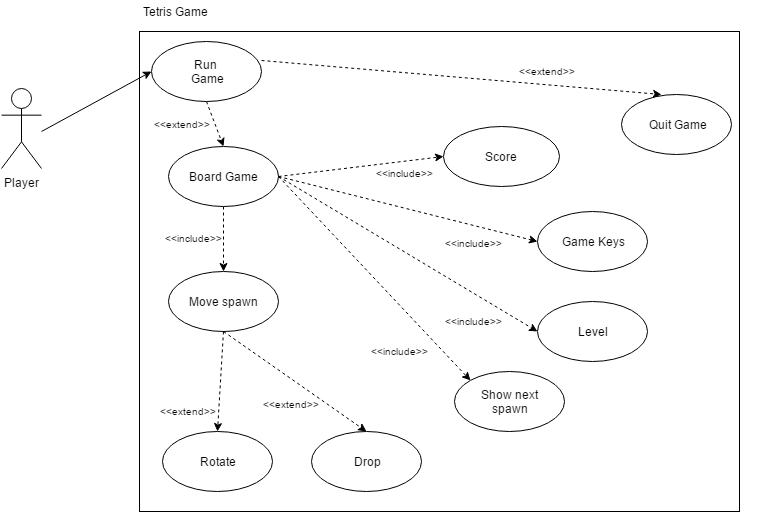
\includegraphics[scale=0.4]{resources/img/use_cases}
	\label{use-cases}
\end{center}

The main use cases are described below: 


\begin{table}[h]
	\centering
%	\caption{Use case 1}
	\label{use-case1}
	\begin{tabular}{|l|l|}
		\hline
		\textbf{Scenario}        & \textbf{Scenario name} \\ \hline
		\textbf{Description}     &                        \\ \hline
		\textbf{Pre-conditions}  &                        \\ \hline
		\textbf{Post-conditions} &                        \\ \hline
		\textbf{Steps}           &                        \\ \hline
		\textbf{Exceptions}      &                        \\ \hline
	\end{tabular}
\end{table}

\subsection{Class model}

\begin{center}
	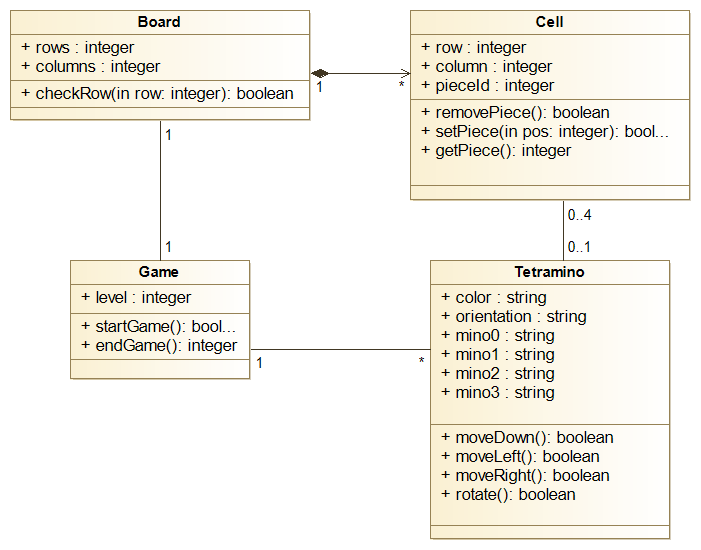
\includegraphics[scale=0.4]{resources/img/uml}
	\label{uml}
\end{center}

\begin{table}[!h]
	\centering
	\label{description-classes}
	\begin{tabular}{|l|l|}
	\hline
	\multicolumn{1}{|c|}{\textbf{Class}} & \multicolumn{1}{|c|}{\textbf{Description}}	\\	\hline
	Game	&	Core model; defines the state variables and operations available to the players.	\\	\hline
	Board	&	Defines a game environment for playing. \\	\hline
	Cell	&	Defines the place on board where each piece of tetrominoes can stay. 	\\	\hline
	Tetromino	&	Defines one piece to play with.	\\	\hline
	\end{tabular}
	\caption{Description of classes}
\end{table}

\section{Formal VDM++ model}

todo

\subsection{Class Game}

todo

\subsection{Class Board}

todo

\subsection{Class Cell}

todo

\subsection{Class Tetromino}

todo

\section{Model validation}

todo

\subsection{Class MyTestCase} 

todo

\subsection{Class TestGame} 

todo

\section{Model verification}

todo

\subsection{Example of domain verification} 

todo

\subsection{Example of invariant verification} 

todo

\section{Conclusions} 

The model that was developed by us covers all the requirements included implicitly on the theme project.
In the final and after model verifications, we all see the game developed in VDM++ like one of the projects more consistent and safer that we have ever developed. 
In addition it is noticed that all the elements of the group have already had contact in the past with the game and they continue to enthuse now with this version developed by us. Maybe in the future we can all add more features to this.
This project took approximately 16 hours to develop.


\section{References}

\begin{itemize}
\item https://en.wikipedia.org/wiki/Tetris
\item http://tetris.com/
\end{itemize}

\newpage
\appendix
\section{Source Code}
\textcolor{red}{maybe not necessary because of section3}
\section{The 7 tetrominoes}

\begin{center}
	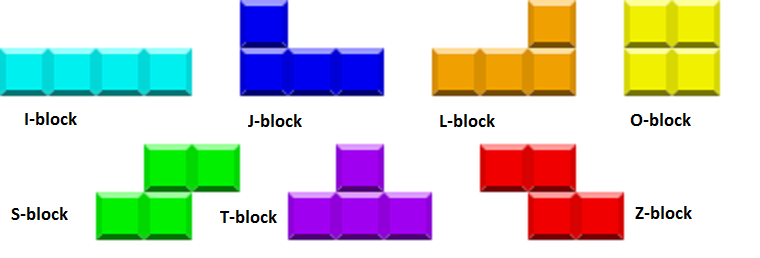
\includegraphics[scale=0.7]{resources/img/tetrominoes}
	\label{tetrominoes}
\end{center}

\end{document}
